\documentclass[11pt]{book}

\usepackage[utf8]{inputenc}
\usepackage[greek, spanish]{babel}
\usepackage{amssymb}
\usepackage{amsmath}
\usepackage[dvips]{graphicx}
\usepackage[dvips]{graphics}
\usepackage{epsfig}

\usepackage{calc}
\usepackage{url}
\usepackage{epsfig}

\usepackage{setspace}
\usepackage{supertabular}
\usepackage{tabularx,colortbl}
\usepackage{makeidx}

\usepackage[left=4cm, bottom=2cm, top=2cm, right=2cm, a4paper]{geometry} 

%Cabeceras y pies del documento (salvo en aquellas páginas donde el estilo sea 'empty', que no tienen
\usepackage{fancyhdr}
\pagestyle{fancy}
\renewcommand{\chaptermark}[1]{\markboth{\scriptsize\MakeUppercase{#1}}{}}
\renewcommand{\sectionmark}[1]{\markright{\tiny\MakeUppercase{#1}}{}}
\fancyfoot{}
\fancyfoot[RO, LE] {\thepage}
\fancyfoot[LO, RE] {\scriptsize Escuela de Ingeniería Informática - Universidad de Oviedo. Alejandro Montes García}
\renewcommand{\footrulewidth}{0.4pt}
%Evita warnings de cabecera
\setlength{\headheight}{15pt}

\makeindex

\hyphenation{fi-na-li-za-do a-de-cua-do o-ca-sio-nal-men-te Pu-bli-co Pro-te-gi-do Pri-va-do Re-tor-no Fi-nal se-cun-da-rios}

\begin{document}

\selectlanguage{spanish} 

\thispagestyle{empty}

\begin{center}
\LARGE
\textbf{UNIVERSIDAD DE OVIEDO}


\vspace{1.5cm}
\begin{tabular*}{5in}{c c c}
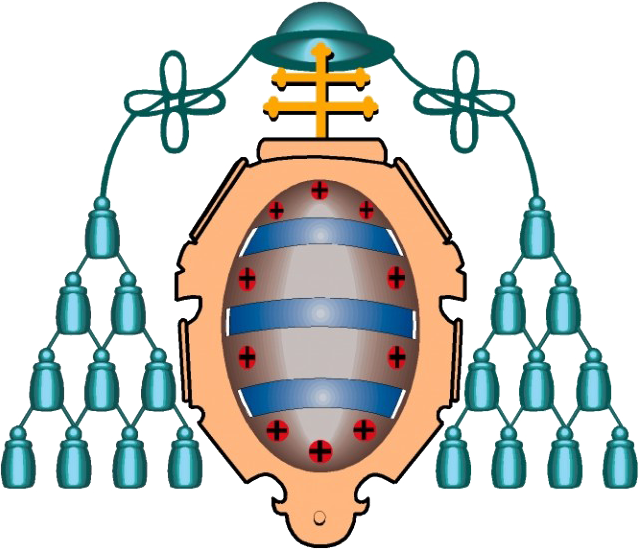
\includegraphics[width=35mm, height=30mm]{img/uniovi} & \hspace{1.75in} & 

\includegraphics[width=30mm, height=30mm]{img/euitio} \\
\end{tabular*}
\end{center}

\vspace{72pt}

\begin{center}
\LARGE
ESCUELA DE INGENIERÍA INFORMÁTICA

\vspace{72pt}

\textbf{PROYECTO FIN DE MÁSTER}

\vspace{72pt}

\noindent ``Arquitectura en web semántica para la recepción, edición y distribución de vídeo digital''

\vspace{104pt}

\normalsize

\begin{tabular}{|p{2.5in}|p{2.5in}|} 
\hline 
\textbf{\vspace{2cm} Vº Bº  del Director del Proyecto} & 
\textbf{AUTOR:} Alejandro Montes García \vspace{1cm} \newline \textbf{DIRECTOR:} Jose María Álvarez Rodríguez \vspace{1cm} \\ 
\hline 
\end{tabular}

\end{center}

\newpage
\thispagestyle{empty}
\mbox{}

\newpage
\thispagestyle{empty}

\section*{Agradecimientos}

\noindent Esta sección no es en absoluto obligatoria, pero es el lugar correcto para dedicar el proyecto a las personas/instituciones/empresas/\dots  que se desee.

\newpage
\thispagestyle{empty}
\mbox{} 

\newpage
\thispagestyle{empty}

\section*{Resumen}

Un texto breve (una cara aproximadamente) que describa qué se ha hecho en el proyecto, sus principales objetivos, la utilidad que se le quiere dar, si está destinado a algún cliente real, aspectos sobre la tecnología usada y cosas similares que permitan hacerse una idea rápida del trabajo realizado. 

Se trata de describir brevemente todos los aspectos más importantes del proyecto destacando en lo posible sus puntos fuertes para permitir comprenderlo fácilmente en una lectura rápida sin tener más referencias del mismo. Por tanto, no debe ser un texto demasiado largo ni complejo.

\newpage
\thispagestyle{empty}
\mbox{}

\newpage
\thispagestyle{empty}
\section*{Palabras Clave}

Palabra1, Palabra2, Palabra3,\dots 

\mbox{}
\mbox{}

\noindent De 5 a 7 palabras\footnote{No necesariamente debe ser una única palabra, pueden ser varias. Por ejemplo, si el proyecto tratase sobre la gestión de calificaciones de Alumnos, una palabra clave válida podría ser ``Expediente Académico''.} clave que mencionen conceptos de capital importancia en el proyecto: Cosas que el proyecto manipula (Ej.: ``Máquinas Expendedoras'', ``Automóviles''), tecnologías usadas (Ej.: J2EE\index{J2EE}, RMI\index{RMI}), utilidad del proyecto (Ej.: Gestión de Existencias), temática (Ej.: Historia Medieval, Aeronáutica) y cosas similares.

\noindent Si finalmente saliesen demasiados términos, conviene hacer una selección de los más relevantes para quedarse con el número indicado. 

\newpage
\thispagestyle{empty}
\mbox{}

\newpage
\thispagestyle{empty}
\section*{Abstract}

\noindent Traducción al inglés del resumen anterior. Conviene hacerlo una vez se tenga la versión definitiva de dicho resumen. Se recomienda consultar al director del proyecto acerca de si considera adecuado que aparezca esta sección.

\newpage
\thispagestyle{empty}
\mbox{}

\newpage
\thispagestyle{empty}

\section*{Keywords}

\noindent Ídem a la sección anterior. Se recomienda consultar al director del proyecto acerca de si considera adecuado que aparezca esta sección.

\newpage
\thispagestyle{empty}
\mbox{}

\newpage
\thispagestyle{empty}

\tableofcontents

\setcounter{tocdepth}{3}

\listoffigures

\chapter{Tecnologías empleadas}
\section{Apache Mahout}
Mahout es una librería de código abierto de Apache que implementa algoritmos de aprendizaje, o \textit{machine learning}. Dentro de este proyecto se utilizará para crear un sistema de recomendación de vídeos al usuario, de modo que este pueda encontrar fácilmente contenido que le interese.
\subsection{Recomendación}
Dentro del mundo de la recomendación, existen dos grandes ramas, la recomendación en base al usuario o la recomendación en base al ítem, en este caso, en base al vídeo.
La recomendación en base al usuario no se basa en la similitud entre dos usuarios en términos de edad, sexo \dots sino que se basa en la similitud entre sus gustos. Típicamente lo que se hace es buscar a sus vecinos (usuarios con gustos más similares) y de cada vecino se busca el vídeo que pueda interesar al usuario inicial. Mahout permite especificar la cantidad de vecinos o que lo calcule él mismo en base a un umbral de similitud.

La recomendación en base al vídeo consiste en evaluar cómo de similar es un vídeo desconocido por el usuario, a los vídeos que le gustan.

Ambos sistemas son eficaces y deberían funcionar bien. A priori no es posible determinar cuál es mejor, no obstante, Mahout proporciona herramientas para saber qué algoritmo recomienda mejor en cuanto se recopilen datos suficientes. Para hacer esto Mahout toma un porcentaje significativo de esos datos y recomienda en base a ello, después toma el resto de datos y comprueba si ha acertado o no.

Puesto que para clasificar un vídeo es necesaria la intervención de un usuario que lo etiquete y categorice, es posible que ese etiquetado sea incorrecto y por tanto, las recomendaciones en base al vídeo fallen, no obstante, en este sistema ese daño se ve minimizado debido a que existirá una moderación de contenido de forma manual.

Ambas formas de recomendación tienen cabida en este proyecto ya que una recomendación en base al usuario permitirá a este encontrar nuevos contenidos que le interesen, y una recomendación en base al vídeo le permitirá encontrar vídeos similares a uno que esté visualizando.

Los datos con los que trabaja Mahout para recomendar son bastante simples, tan solo consiste en asociar usuarios e ítems, y opcionalmente, a esta asociación se le da un valor de preferencia. En el caso de Freews se podrían almacenar estas asociaciones sin valor de preferencia en base a los vídeos que un usuario visita (feedback implícito), se podría asignar un valor de preferencia si el usuario puntúa un video (feedback explícito) o se podrían combinar feedback implícito y explícito. Ignorar el valor de preferencia puede ser bueno ya que se optimiza el consumo de memoria, además de que los usuarios no suelen puntuar vídeos o si lo hacen suelen ir a los extremos (muy bueno o muy malo) por lo que de implementar feedback explícito lo más recomendable es hacer algo del estilo ``Me gusta'' o ``No me gusta''.

Además de la recomendación en base al usuario y en base al video, Mahout implementa otros algoritmos como Slope One que consiste en suponer que existe una relación lineal entre la puntuación de los videos, SVD, interpolación linal basada en objetos, y recomendación basada en clústers.

Internamente Mahout reinventa la forma de guardar las preferencias en memoria para ocupar menos, utilizando clases como \texttt{PreferenceArray} y sus implementaciones.

Para determinar la similitud entre dos objetos, ya sea en una recomendación en base al usuario o en una en base al vídeo, Mahout implementa varios algoritmos como el coeficiente de correlación de Pearson, la distancia euclídea, el del coseno, el coeficiente de correlación de Spearman o el Coeficiente de Tanimoto si se ignoran los valores de preferencia. Todos ellos son estadísticos empleados para calcular la dependencia o la relación lineal entre dos valores.
\section{Apache Maven}
Maven es una herramienta de gestión de proyectos. Basándose en un POM (\textit{Project Object Model}), Maven puede gestionar la construcción y documentación de un proyecto de forma centralizada \cite{maven}.
\section{Apache Solr}
Apache Solr es una plataforma de código abierto de Apache que sirve para realizar búsquedas. Sus características principales incluyen: búsqueda textual completa, resaltado de resultados, búsqueda de características, clustering dinámico, integración con bases de datos, manejo de documentos de texto enriquecido y búsqueda geoespacial \cite{solr}.
\section{FFmpeg}
FFmpeg es una plataforma para grabar, convertir y reproducir vídeos. FFmpeg es software libre distribuido bajo licencia GPL \cite{ffmpeg}. FFmpeg se usará en Freews para la generación de noticiarios a partir de clips de vídeo junto con cabeceras y ráfagas.
\section{MongoDB}
MongoDB es una base de datos escalable, de alto rendimiento, de código abierto y NoSQL. Está orientada a documentos JSON, permite indexar por cualquier atributo, incorpora sistemas de replicación, alta disponibilidad, y escalado horizontal sin comprometer su funcionalidad \cite{mongodb}.
\section{Struts}
Struts es un \textit{framework} de software libre sobre el que construir aplicaciones web en Java bajo el patrón MVC (\textit{Model View Controller}) \cite{struts}. Se utilizará Struts para el desarrollo de un cliente web de la aplicación.
\section{Spring}
Spring es un \textit{framework} para Java que permite mejorar el desarrollo de una aplicación \cite{spring}. En este proyecto se usará Spring para inyectar dependencias, mejorando el desacoplamiento entre las capas de presentación, lógica y persistencia.
\chapter{Diseño del sistema}
\section{Despliegue del sistema}
El sistema consta de diversos componentes. Por un lado, el cliente web hecho con Struts está desplegado en un servidor Tomcat. Este cliente se conecta a varias bases de datos NoSQL MongoDB para recuperar datos. Para realizar búsquedas más elaboradas, el cliente web se conecta primero a Solr y recupera los IDs de los vídeos que formarán parte del resultado de la busqueda, posteriormente se conecta a una de las bases de datos para recuperar la información completa de los distintos clips.

El cliente web, a su vez, hace uso de FFmpeg para tratar los vídeos, también se conecta a la API de Facebook para interactuar con esta red social.

Esta estructura se resume en el siguiente diagrama de despliegue:

\begin{figure}[ht]
\centering
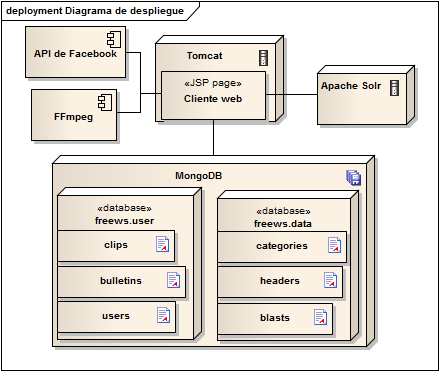
\includegraphics[scale=0.75]{img/uml/despliegue}
\caption{Diagrama de despliegue}
\label{uml:despliegue}
\end{figure}
\section{Diseño del cliente  web}
Para el cliente web se ha utilizado el \textit{framework} Struts en su versión 2.3.4. Se ha estructurado el código Java utilizando un patrón \textit{layers} distinguiendo entre presentación, donde estarán las \textit{action} de Struts, negocio, donde se implementará la lógica de la aplicación y persistencia, donde se interactuará con la base de datos, en este caso MongoDB. El desacoplamiento entre capas es total gracias al uso de Spring, que permite especificar las clases que implementan los interfaces definidos con tan solo hacer un cambio en un archivo XML.

Además de ello existe un paquete de infraestructura donde estarán las clases de log, otro con un modelo anémico de los objetos Java que se utilizarán en el modelado de la aplicación y por último otro paquete de utilidad en el que hay clases encargadas en interactuar con FFmpeg, con Facebook, etc\dots.

Para clarificar este diseño, se muestra el siguiente diagrama de paquetes:

\begin{figure}[ht]
\centering
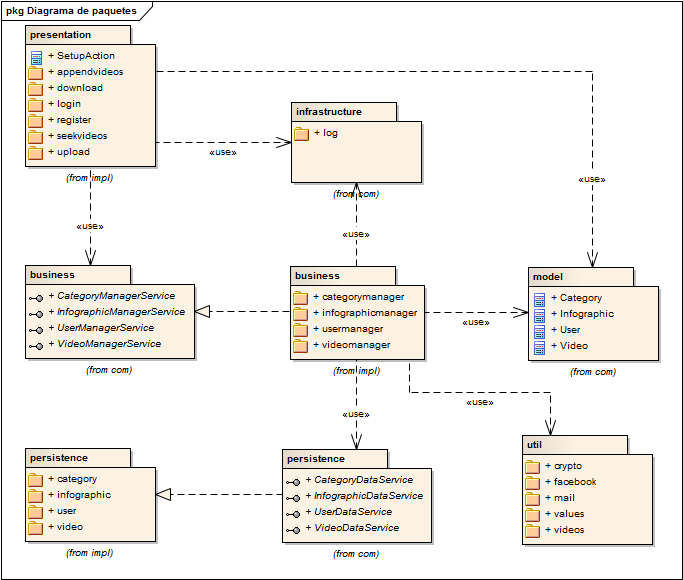
\includegraphics[scale=0.62]{img/uml/paquetes}
\caption{Diagrama de paquetes}
\label{uml:paquetes}
\end{figure}
\chapter{Manual de instalación}
Existen tres aplicaciones a instalar: El cliente web, el servidor Apache Solr y la base de datos. Estas tres instalaciones se han hecho en un servidor Windows Server 2008 R2.

\paragraph{Base de datos MongoDB}
La base de datos puede descargarse de la página web \url{http://www.mongodb.org/downloads}. 

Para ejecutar la base de datos basta con abrir un nuevo terminal, situarse en la carpeta bin del contenido descargado y ejecutar la orden \texttt{mongod}. Deberá especificarse una carpeta existente donde se alojará o donde está actualmente alojada la base de datos, eso se hace con el parámetro \texttt{--dbpath} por lo que si la carpeta de la base de datos está en el mismo directorio que el archivo \texttt{mongod.exe}, y dicha carpeta se llama \textit{freews}, la orden será: \texttt{mongod --dbpath=freews}.

\paragraph{Servidor Apache Solr}
El servidor Apache Solr puede descargarse de \url{http://archive.apache.org/dist/lucene/solr/3.6.0/}.

Para lanzar la ejecución de Apache Solr simplemente hay que ejecutar el fichero \texttt{example\textbackslash start.bat}. No obstante, antes se debera sustituir el esquema de Solr por uno que se ajuste al esquema del proyecto, para ello basta con reemplazar el fichero \texttt{example\textbackslash solr\textbackslash \\conf\textbackslash schema.xml} por el \texttt{schema.xml} proporcionado. Una vez ejecutado Solr se deben borrar los datos de ejemplo. Para ello se puede utilizar la herramienta \texttt{example\textbackslash example\textbackslash post\\.jar} con un fichero XML que contenga el texto \texttt{<delete><query>*:*</query></delete>}.

\paragraph{Cliente web}
Para instalar el cliente web es necesario un servidor Tomcat que se puede descargar de \url{http://tomcat.apache.org/download-70.cgi}.

A la instalación por defecto de Tomcat hay que hacerle dos cambios en el fichero \texttt{conf\textbackslash server.xml}. En la línea donde se define el \textit{connector} del puerto 8080, hay que cambiar el puerto al 80 y añadir el atributo \texttt{URIEncoding=``UTF-8''}. Una vez hecho esto basta con copiar el archivo \texttt{Freews.war} a la carpeta webapps. Se creará un directorio Freews, dentro del cual, en la carpeta \texttt{WEB-INF\textbackslash classes} hay un fichero llamado \texttt{applicationContext.xml} en el que se definirán las clases que implementan la capa de negocio y persistencia, asi como otros aspectos como la ruta al directorio donde está FFmpeg, etc\dots Es posible que haya que hacer cambios en ese fichero, así como el \texttt{struts.xml} donde se define el directorio por defecto de subida de archivos. Una vez hecho esto, el proyecto está listo para ser ejecutado. Se pueden cargar unos datos de ejemplo accediendo en el navegador a la url \url{http://localhost/Freews/Setup}.
\begin{thebibliography}{9}
\bibitem{mia} Owen Sean; Anil, Robin; Dunning Ted, Friedman, Ellen. Mahout in action. Manning 2010. ISBN 9781935182689.
\bibitem{maven} Maven - Apache Maven. \url{http://maven.apache.org/} Consultado el 13 de julio de 2012.
\bibitem{solr} Apache Lucene - Apache Solr. \url{http://lucene.apache.org/solr/} Consultado el 13 de julio de 2012.
\bibitem{ffmpeg} FFmpeg. \url{http://ffmpeg.org/} Consultado el 13 de julio de 2012.
\bibitem{mongodb} MongoDB. \url{http://www.mongodb.org/} Consultado el 13 de julio de 2012.
\bibitem{struts} Struts. \url{http://struts.apache.org/} Consultado el 13 de julio de 2012.
\bibitem{spring} SpringSource. \url{http://www.springsource.org/} Consultado el 13 de julio de 2012.
\end{thebibliography}

\newpage
\thispagestyle{empty}
\mbox{}

\end{document}


